


\documentclass[main]{subfiles}

\begin{document}

\chapter{Background Research}

\section{Scope of Research} \label{sec:scoperesearch}

In Chapter 1 (``Approaches to Interpretability'') a brief overview of feature attribution methods was provided with reference to a distinction between model-specific and model-agnostic methods. This is a common distinction in the literature and was also used to guide research in this project. The panel of methods chosen for evaluation ultimately consisted of a balanced selection from both approaches. 

A major difficulty of this project was distilling the broad literature on these methods however. For the model-specific (neural network) family, different angles are commonly taken to calculate feature ``relevance'' or importance. These include generally:
\begin{itemize}
\item \textbf{Gradient-based} methods, saliency maps and output sensitivity methods
\item \textbf{Backpropagation-based} methods or `importance signal' visualisations (such as activations in a hidden layer)
\item \textbf{Perturbation-based} methods and use of occlusion masks in the input space
\end{itemize}

This categorisation is based on two recent papers that make similar categorisations of explanation approaches  \cite{deeplift} \cite{patternnet}. In this chapter a broad selection of methods based on traction over time, current popularity and representativeness of approach are described, though the reader should note there are many more methods under each of those three than have been described here.

For model-agnostic methods, perturbation-based and surrogate model approaches are considered. Again the selection was based on traction and literature popularity.

First reviewed are traditional, visual approaches to interpretability to provide context to the task of feature attribution. After the exploration of feature attribution methods, a review of existing evaluation metrics and comparison studies is provided.

\subsection*{Terminology}
A note on terminology is that all methods are variously referred to as \textit{attribution} methods in this project for any projection on the input space that causes an explanation to take place. Goodfellow, Kim, et al. refer to the broad category of ``visualisation and attribution methods aimed at interpreting trained models'' as \textit{saliency} methods instead \cite{sanity}. A \textit{saliency map} is widely-used as a `catch-all' term to refer to input space projections (individual explanations themselves) in the context of interpreting deep neural networks for image data (\cite{sanity}). However they also refer to a specific gradient-based method (\textbf{cite below}). 

There seems to be little consensus around terminology. Some researchers (\cite{patternnet}) describe attribution methods as a subclass of explanation techniques where contribution scores are specifically calculated for each input feature (i.e. excluding higher level `patterns' which cause  neuron activations, as in Zeiler \& Fergus (\cite{zeilerfergus2013}) (Section \textbf{X}) or the back-propagation class generally). 

In summary, attribution methods are used here as a general term, but can refer specifically to contribution `calculators', and saliency methods/maps is widely used in the context of neural networks and image data.

\section{Traditional Approaches}

\subsection{Feature Projection}
Visualisation tools for high-dimensional data are a popular way to gauge insight into expected model behaviour.  These pre-learning, exploratory data analysis techniques include mathematical reductions like PCA and probabilistic techniques like t-SNE,  projecting high-dimensional examples that are `similar' into a visualisable 2D or 3D space \cite{tsnepaper} (Figure \ref{tsneimg}).

\begin{figure}[h]
\centering
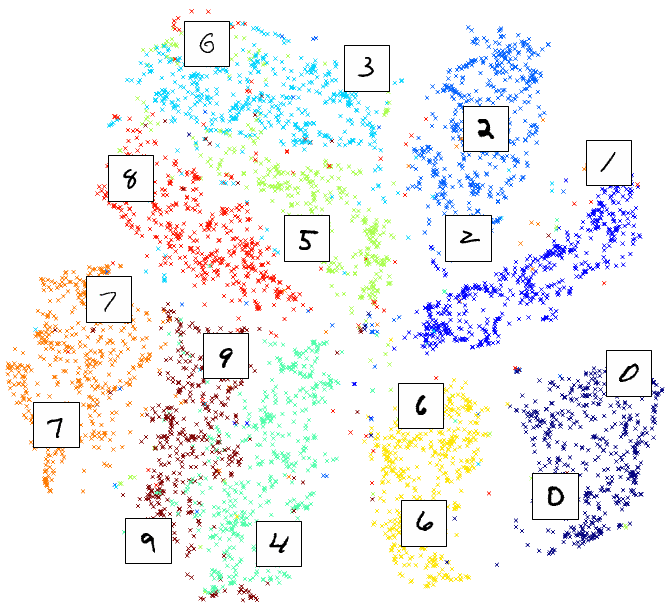
\includegraphics[scale=0.2]{tsne.png}
\caption{2D embedding of 70,000 handwritten digits (0-9) from MNIST \cite{tsne}}
\label{tsneimg}
\end{figure}

Other methods of clustering and dimensionality reduction are also widely used for interpreting data, and although useful for gaining an intuition on relationships between features, they are not suited for explaining model behaviour as they examine only the input space itself. 

\subsection{Partial Dependence Plots}

A partial dependence plot (PDP) is a tool to demonstrate the marginal effect of one or two features on a prediction outcome. It was proposed by Friedman in 2001 to interpret and visualise the features that his gradient boosting machine relied upon (though it is limited to 1 or 2 input features such that it can be displayed) \cite{pdp1}. A partial dependence function $\widehat{f_{xs}}$ can be calculated for some desired set of features S, by marginalising the model output over the set of `complement` features C (all other features):
\begin{align}
\widehat{f_{xs}}=\int \widehat{f}(x_{s}, x_{c})dP(x_{c})
\end{align}
It can be approximated with a Monte Carlo method. Friedman believed in 2001 that these might be used to help interpret ``any black box prediction method'' such as NN and SVM architectures, and that, ``[...] when there are a large number of predictor variables, it is very useful to have a measure of relevance to reduce the potentially large number of variables to be considered" \cite{pdp1}. The mentioned relevance measure was defined only in the context of the decision trees which constituted the paper's gradient boosting machine. Certainly, PDPs are suited for the low-dimensional feature spaces that were imagined in the pre-deep learning era, and are less suitable for high-dimensional input spaces such as in image classification. They are also restricted by an unrealistic assumption of independence among features.

\section{Model-Specific Methods}
Deep learning's reputation for lack of transparency has led to many attempts to explain the predictions of complex NN architectures. This section examines representative attribution methods from the gradient-based, backpropagation-based and perturbation-based approaches overviewed in Section \ref{sec:scoperesearch}, with some emphasis on those developed in the context of CNNs (i.e. image data).


\subsection{Backpropagation-Based}

This class of methods try to isolate an internal model signal, such as neuron activations in a target hidden layer, and map these signals back into the input pixel space. Zeiler and Fergus (2014) introduced the motivation for signal backpropagation as, `[...] showing what input pattern originally caused a given activation in the feature maps" \cite{zeiler}. 

\subsubsection{Feature Visualisation}
First described is the feature visualisation approach, which is a technique to visualise inner model workings. This is not a true feature attribution method, as it is visualising internal `trained features' instead of attributing the contributions of input features, though it is briefly discussed for its relevance to formulations in the backpropagation family and to gradient-based methods as well.

The success of  visualisation approach is a technique to explore internal model workings, via visualisations of units within a model. These units can be layers, individual convolutional channels (or feature maps) or even an individual neuron like out an output class neuron

%https://christophm.github.io/interpretable-ml-book/cnn-features.html#fn73

\subsubsection{DeConvNet}


In their creation of class-based saliency maps (Section 1.3.1) Simonyan et al. showed that DeconvNet-based reconstruction of the input to a hidden is equivalent to computing the gradient of visualised neuron activations with respect to that input \cite{saliencyII}.

Guided BackProp

Layer-wise Relevance Propagation 

DeepTaylorDecomposition
%http://www.heatmapping.org/deeptaylor/





\subsection{Gradient-Based}
These methods aim to explain a class output in terms of sensitivity in the input space by relying on a gradient function of the output. The goal is to find the input features that make that prediction more or less confident.  For an output prediction of `tree' for example, they seek to answer ``what makes a tree more/less a tree?''.

\subsubsection{Saliency Maps}
An early formulation of a local explanation method was provided by Baehrens et al. (2010) for any nonlinear classification algorithm \cite{saliencyI} (though developed in the context of Bayesian classification). The local explanation gradient vectors that this paper devised were based on class probability gradients, characterising how much a data point has to be moved for a predicted label to change. Simonyan et al. (2014) later applied a similar idea to CNNs to create `class saliency maps' specific to a given image and class \cite{saliencyII}. 

\begin{figure}[h]
\centering
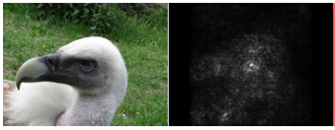
\includegraphics[scale=0.8]{saliency.png}
\caption{(From \cite{saliencyII}) Example of an image-specific class saliency map.}
\label{tsneimg}
\end{figure}

The formulation is based on finding the derivative of an output class with respect to an input image via back-propagation. The authors also formulate a method to generate an image that maximises the output class score for a particular class, to visualise the model's `interpretation' of a class. This paper sparked popularity for saliency maps and further interest in creating explanations from network gradients. Note that a drawback of saliency maps is that noisy images can be produced when a model does not distinguish between objects that are being predicted and nearby objects that are associated (i.e. a tree with leaves, in an image of a bird).

\subsubsection{Class Activation Maps}
Another visual approach aimed at understanding the behaviour of CNNs was introduced by Zhou et al. (2015) and 


GradCAM
gradcam efficient variation https://arxiv.org/abs/1911.11293

%Occlusions for Effective Data Augmentation in Image Classification
%https://arxiv.org/abs/1910.10651

%Understanding Deep Networks via Extremal Perturbations and Smooth Masks
%https://arxiv.org/abs/1910.08485

%Interpretable Explanations of Black Boxes by Meaningful Perturbation
%http://openaccess.thecvf.com/content_ICCV_2017/papers/Fong_Interpretable_Explanations_of_ICCV_2017_paper.pdf


Integrated Gradients (ref DeepLIFT)

SmoothGrad


\subsection{Perturbation-Based}

occlusion and ablation

occlusion mask, zeiler and fergus

\section{Model-Agnostic Methods}


"While we have made a case for model agnosticism, this
approach is not without its challenges. For example,
getting a global understanding of the model may be hard
if the model is very complex, due to the trade-off between
flexibility and interpretability. To make matters worse, local
explanations may be inconsistent with one another, since a
flexible model may use a certain feature in different ways
depending on the other features. In Ribeiro et al. (2016)
we explained text models by selecting a small number
of representative and non-redundant individual prediction
explanations obtained via submodular optimization, similar
in spirit to showing prototypes (Kim et al., 2014). However,
it is unclear on how to extend this approach to domains such
as images or tabular data, where the data itself is not sparse.
In some domains, exact explanations may be required (e.g.
for legal or ethical reasons), and using a black-box may
be unacceptable (or even illegal). Interpretable models
may also be more desirable when interpretability is much
more important than accuracy, or when interpretable models
trained on a small number of carefully engineered features
are as accurate as black-box models."  Model-Agnostic Interpretability of Machine Learning



\subsection{Perturbation-Based}
Both gradient and backpropagation-based methods operate under the assumption that propagating an output signal, back through a classifier model, is a means to explain how a relevant signal was originally encoded in an input \cite{patternnet}. An alternative approach is to treat the model as more of a black box, by perturbing the input space (such as occluding important parts) to study the effect on the output. Changes in output would reveal that occluded parts of the input are important in a prediction. 

"The problem of attribution is concerned with identifying the parts of an input that are responsible for a model's output. An important family of attribution methods is based on measuring the effect of perturbations applied to the input"




\subsection{Surrogate Models}
some overlap with perturbation-based methods for how they are trained

%https://christophm.github.io/interpretable-ml-book/lime.html


variants of lime include KL-lime

\section{Evaluation Metrics}


%https://arxiv.org/abs/1907.09701
%https://distill.pub/2020/attribution-baselines/

%https://arxiv.org/pdf/1711.00867.pdf

%sanity checks for saliency maps
%https://arxiv.org/pdf/1810.03292.pdf

%unreliability of saliency methods
%https://arxiv.org/pdf/1711.00867.pdf

%https://medium.com/swlh/breaking-down-the-black-box-39403b0f64a3

%IOU: Network Dissection: Quantifying Interpretability
%https://arxiv.org/abs/1704.05796

%\cite{saliencyII}
%Section 3.2 Weakly Supervised Object Localisation
%weakly supervised object localisation from Saliency Maps
%used a segmentation algorithm and entered their saliency
% map into ILSVRC-2013 localisation challenge


\section{Existing Explanation Frameworks}

%Skater - a unified framework for model-agnostic interpretation --> global and local
%DeepExplainer

%TorchRay https://github.com/facebookresearch/TorchRay

\section{Existing Evaluation Studies}

Comparisons


\end{document}
